\documentclass{article} 
\usepackage{tikz}
\usepackage{listings}
\usepackage{graphicx}

\begin{document} 

\begin{figure}
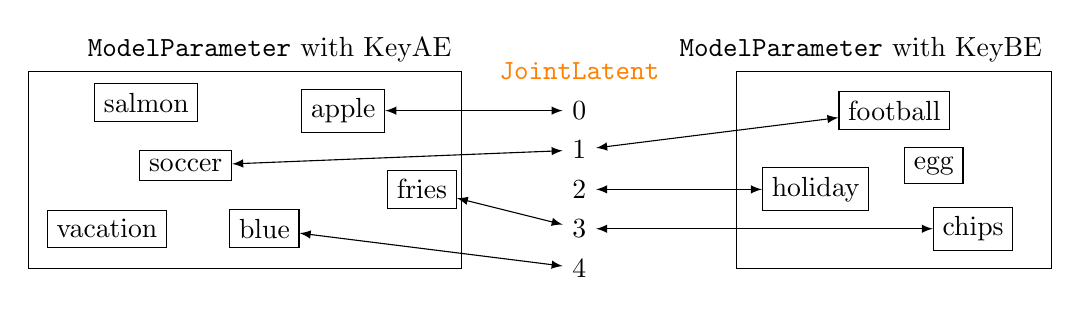
\begin{tikzpicture}
  \node[draw=black](vacation) at (-6,0) {vacation};
  \node[draw=black](fries)    at (-2,0.5) {fries};
  \node[draw=black](soccer)   at (-5,0.8) {soccer};
  \node[draw=black](apple)    at (-3,1.5) {apple};
  \node[draw=black](blue)     at (-4,-0.0) {blue};
  \node[draw=black](salmon)   at (-5.5,1.6) {salmon};
  \draw (-7, -0.5) rectangle (-1.5, 2) node [above left] {\texttt{ModelParameter} with KeyAE} ;
  
  
  \node[draw=black](holiday) at (3,0.5) {holiday};
  \node[draw=black](chips) at (5,0.0) {chips};
  \node[draw=black](football) at (4,1.5) {football};
  \node[draw=black](egg) at (4.5,0.8) {egg};
  \draw (2, -0.5) rectangle (6, 2) node [above left] {\texttt{ModelParameter} with KeyBE} ;
 
  \node[orange] at (0, 2) {\texttt{JointLatent}};
  \node (0) at (0,1.5) {0};
  \node (1) at (0,1.0) {1};
  \node (2) at (0,0.5) {2};
  \node (3) at (0,0.0) {3};
  \node (4) at (0,-.5) {4};

  \draw[latex-latex] (soccer)--(1);
  \draw[latex-latex] (apple)--(0);
  \draw[latex-latex] (fries)--(3);
  \draw[latex-latex] (blue)--(4);
  
  
  \draw[latex-latex] (football)--(1);
  \draw[latex-latex] (chips)--(3);
  \draw[latex-latex] (holiday)--(2);

  %\draw (-0.5, -0.5) rectangle (1.5, 1.5) node [above left] {Key1} ;
\end{tikzpicture}
\caption{Mapping of latent parameters of two individual \texttt{ModelParameter} collections to shared list of latent parameters.}
\end{figure}

\section{Individual \texttt{ModelParameter} collections are not sorted/ordered}

\begin{itemize}
  \item represented by wildy arranged nouns
  \item Why? Because they can!
\end{itemize}


\section{Only latent parameters are relevant for the joined list}

The whole purpose is the mapping of a latent parameter vector for maths algorithms
to (multiple) named parameters of \texttt{ModelParameter}. If a parameter is not 
latent, it does not need to be mapped.

\section{Adding parameters}

\begin{lstlisting}[basicstyle=\ttfamily, language=python]
latent.add("apple", key="KeyAE") 
entry = latent.add("soccer", "KeyAE")
latent.add_shared(entry, "football", "KeyBE")

latent.add("holiday", "KeyBE")
entry = latent.add("fries", key="KeyAE")
assert entry == 3
latent.add_shared(entry, "chips", "KeyBE")

latent.add("blue", "KeyAE"))
\end{lstlisting}

\section{Access}

\begin{itemize}
  \item \texttt{parameter(0)} $\to$ KeyAE, apple
  \item \texttt{parameter(1)} $\to$ KeyAE: soccer, KeyBE: football
  \item \texttt{index\_of(holyday, KeyBE)} $\to$ 2
  \item \texttt{index\_of(holyday, KeyAE)} $\to$ RuntimeError
  \item \texttt{indices\_of("KeyBE")} $\to 1,2,3$
  \item \texttt{indices\_of("KeyBE", "chips")} $\to 3$
  \item \texttt{indices\_of("KeyBE", "egg")} $\to$ RuntimeError
\end{itemize}

\section{Update}

Calling \texttt{update(numbers)} will leave the original \texttt{ModelParameter} 
collections untouched and instead return a modified copy.

\end{document}
